\chapter{Materiais e Métodos}
\label{cap:metodologia}

Utilizando como base os conceitos previamente abordados, este Capítulo descreve os ambientes de \textit{benchmark} utilizados para experimentação, o funcionamento do algoritmo utilizado e os testes executados. Primeiramente, são apresentados os objetivos do agente nos ambientes escolhidos e como é configurada a observação e a recompensa, assim como o espaço de ações e a duração do episódio. Em seguida, o algoritmo PPO é retomado e modificado para incluir o módulo de motivação intrínseca. O funcionamento geral dos passos do algoritmo são descritos em mais detalhes e a arquitetura das redes neurais utilizada é apresentada. Por fim, os testes são descritos e as hipóteses deste trabalho são estabelecidas, assim como o comportamento esperado de cada métrica a ser analisada.

% - - - - - - - - - - - - - - - - - - - - - - - - - - - - - - - - - - -

\section{OpenAI Gym}
\label{sec:gym}

\begin{figure}[hb]
 \centering
  \subfigure[CartPole.]
   {
    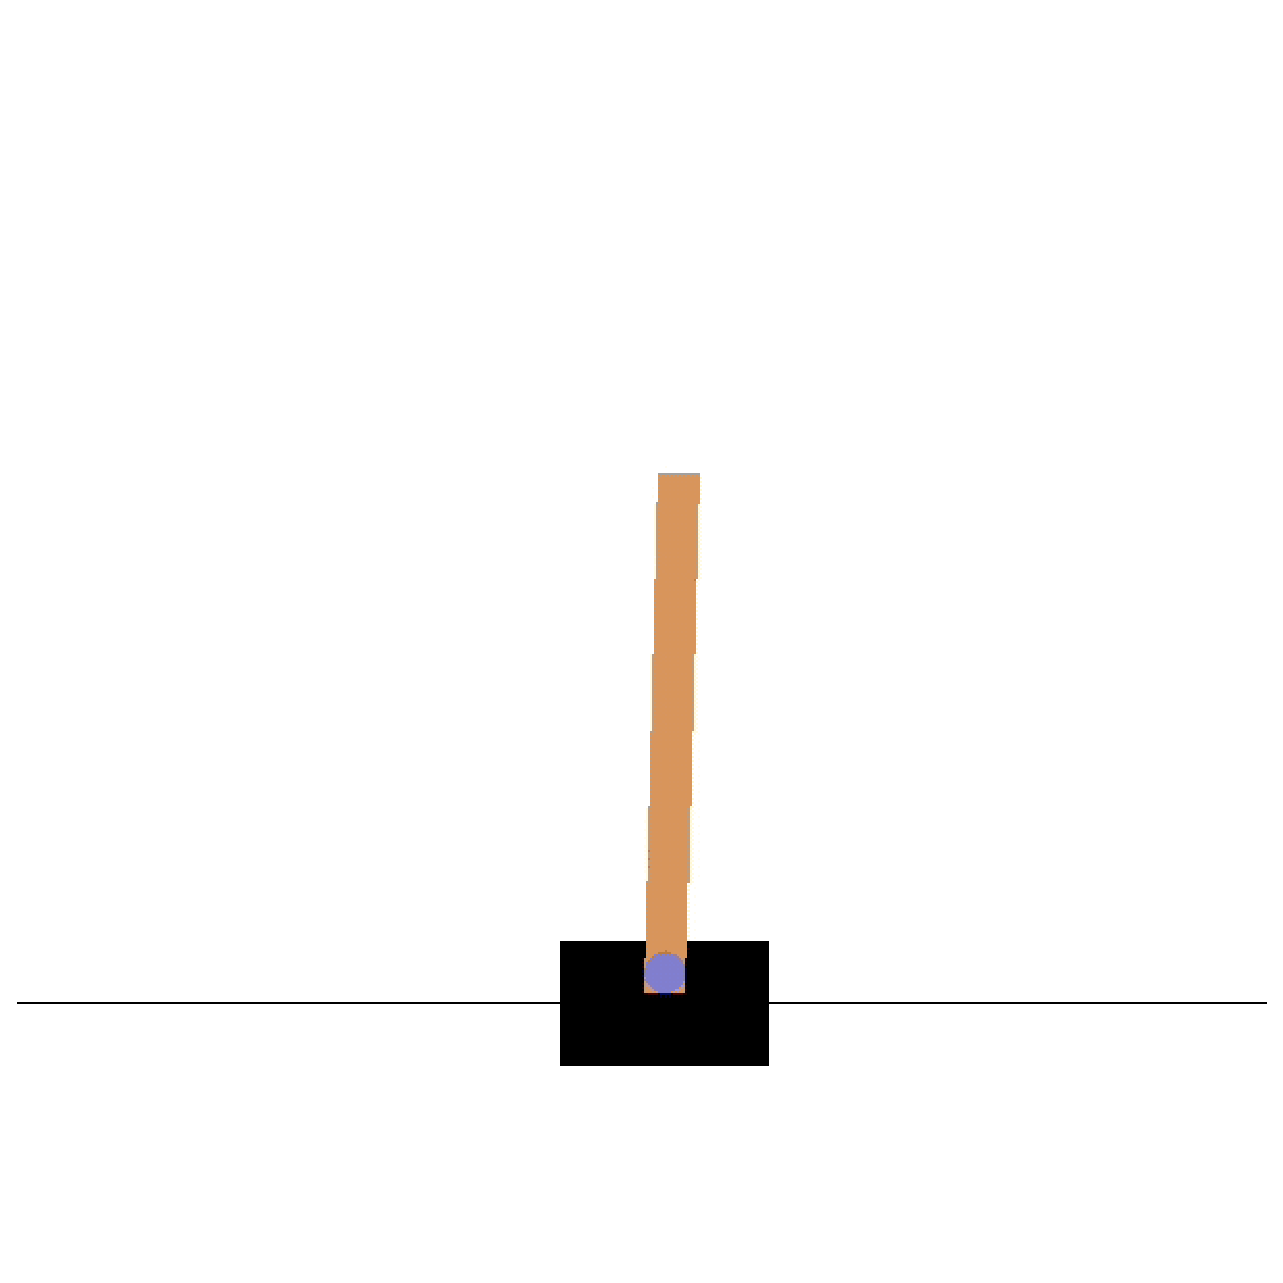
\includegraphics[width=0.35\textwidth]{./fig/cartpole-0}
    \label{subfig:cartpole}
   } \qquad
  \subfigure[HandManipulateBlock.]
   {
    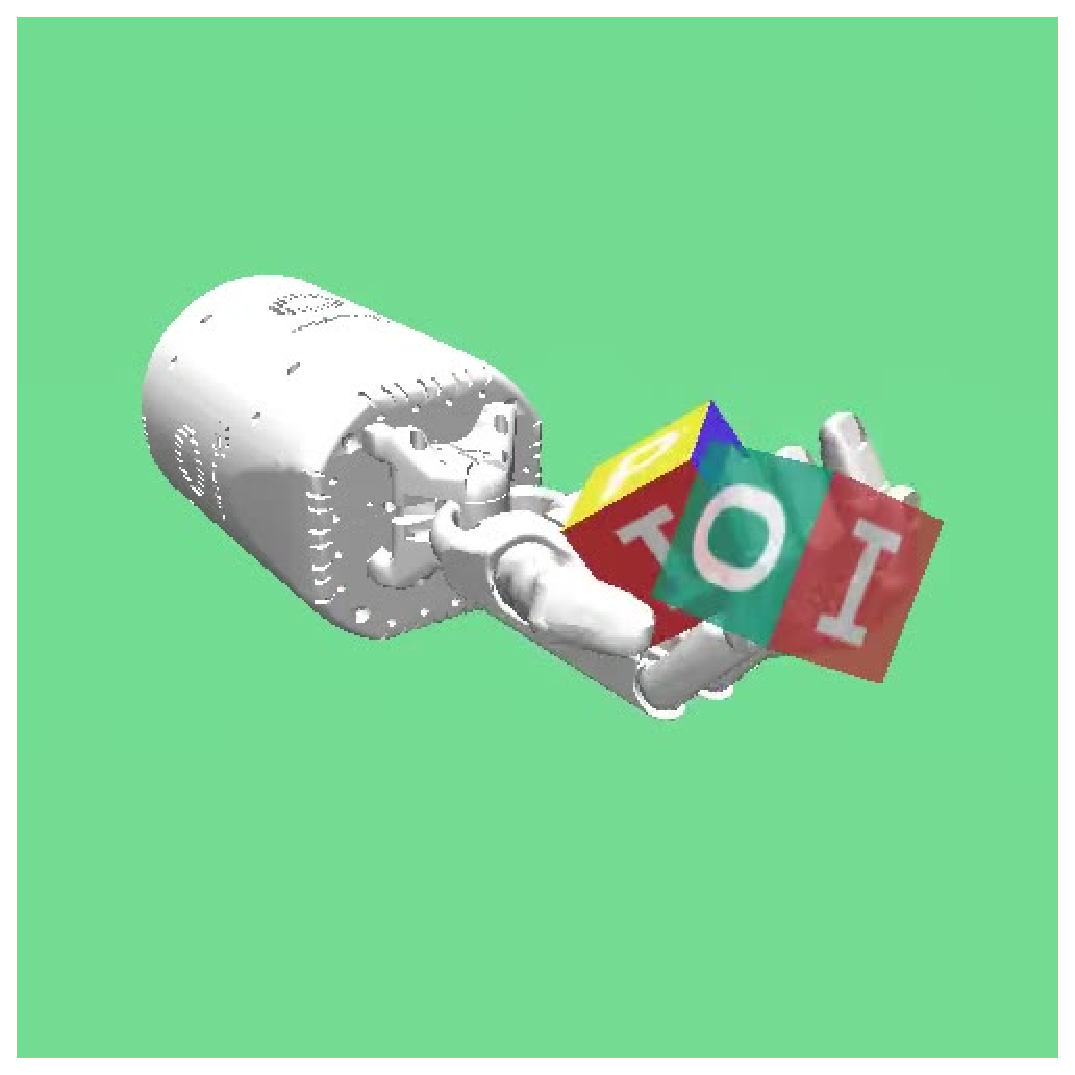
\includegraphics[width=0.35\textwidth]{./fig/handmanipulate}
    \label{subfig:handmanipulate}
   }
   \captionsetup{width=1\textwidth}
   \caption[Ambientes do Gym.]{Ambientes do Gym. Em {\subref{subfig:cartpole}}, o agente deve equilibrar a estaca selecionando ações entre [esquerda, direita]. Em {\subref{subfig:handmanipulate}}, o agente deve posicionar o bloco opaco como mostra o bloco translúcido de exemplo, selecionando valores de torque para cada junta da mão.}
  \label{fig:gymenvs}
\end{figure}

O OpenAI Gym \cite{gym} é uma ferramenta de \textit{benchmark} para algoritmos de aprendizado por reforço que tem como objetivo ser agnóstico em relação à estrutura dos agentes e manter uma interface amigável e comum a seus diversos ambientes. O Gym inclui ambientes que variam desde problemas simples, como o famoso \textit{CartPole} (Figura \ref{subfig:cartpole}), até simulações de mãos robóticas, como o \textit{HandManipulateBlock} (Figura \ref{subfig:handmanipulate}).

Para os testes deste trabalho, foram escolhidos ambientes de manipulação robótica \textit{FetchReach}, \textit{FetchPush}, \textit{FetchPickAndPlace}, ilustrados pela Figura \ref{fig:fetchenvs}. A escolha desses ambientes possibilita a avaliação da aplicabilidade de técnicas similares a apresentada neste trabalho em manipuladores reais.

\begin{figure}[ht]
 \centering
  \subfigure[FetchReach.]
   {
    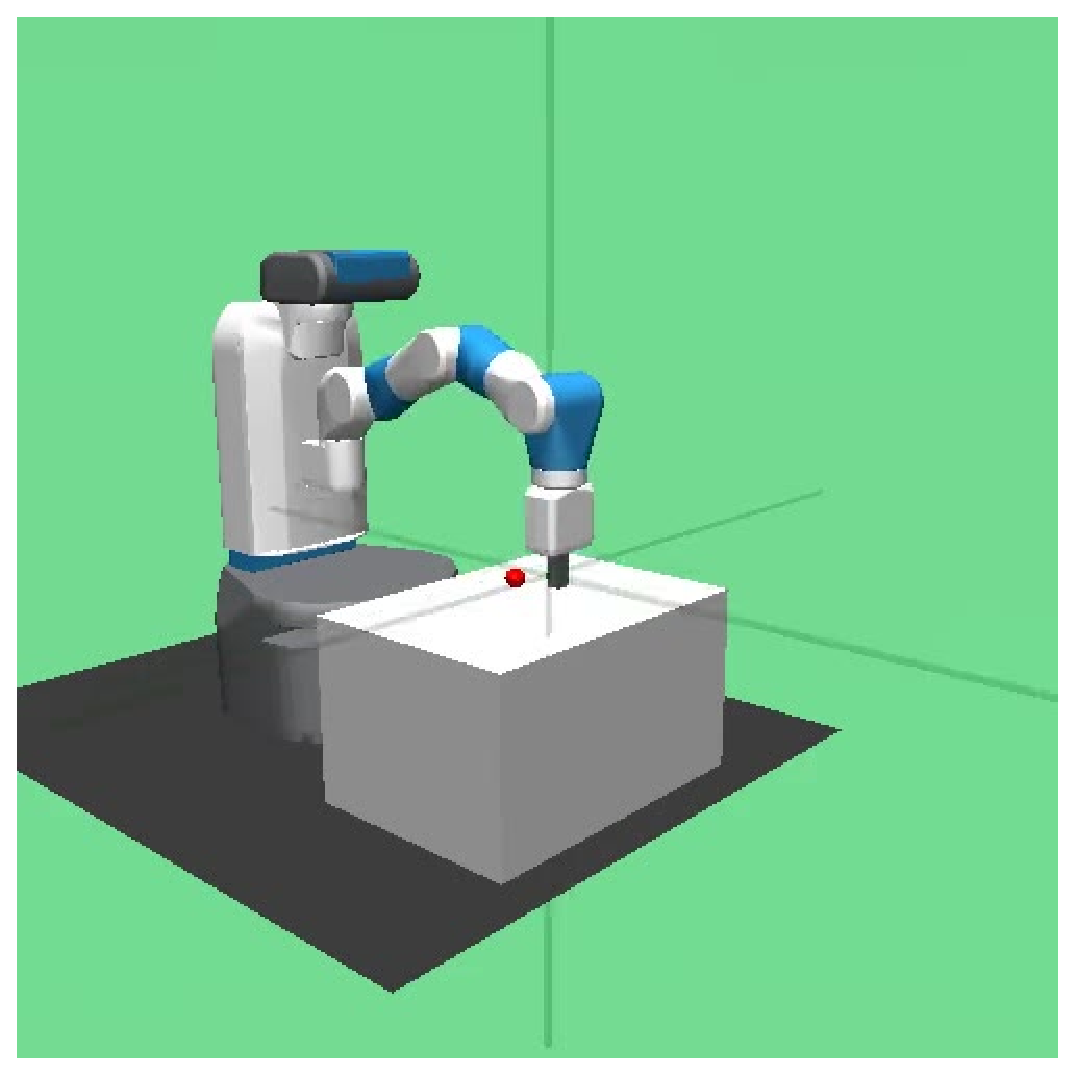
\includegraphics[width=0.3\textwidth]{./fig/fetchreach}
    \label{subfig:fetchreach}
   }
  \subfigure[FetchPush.]
   {
    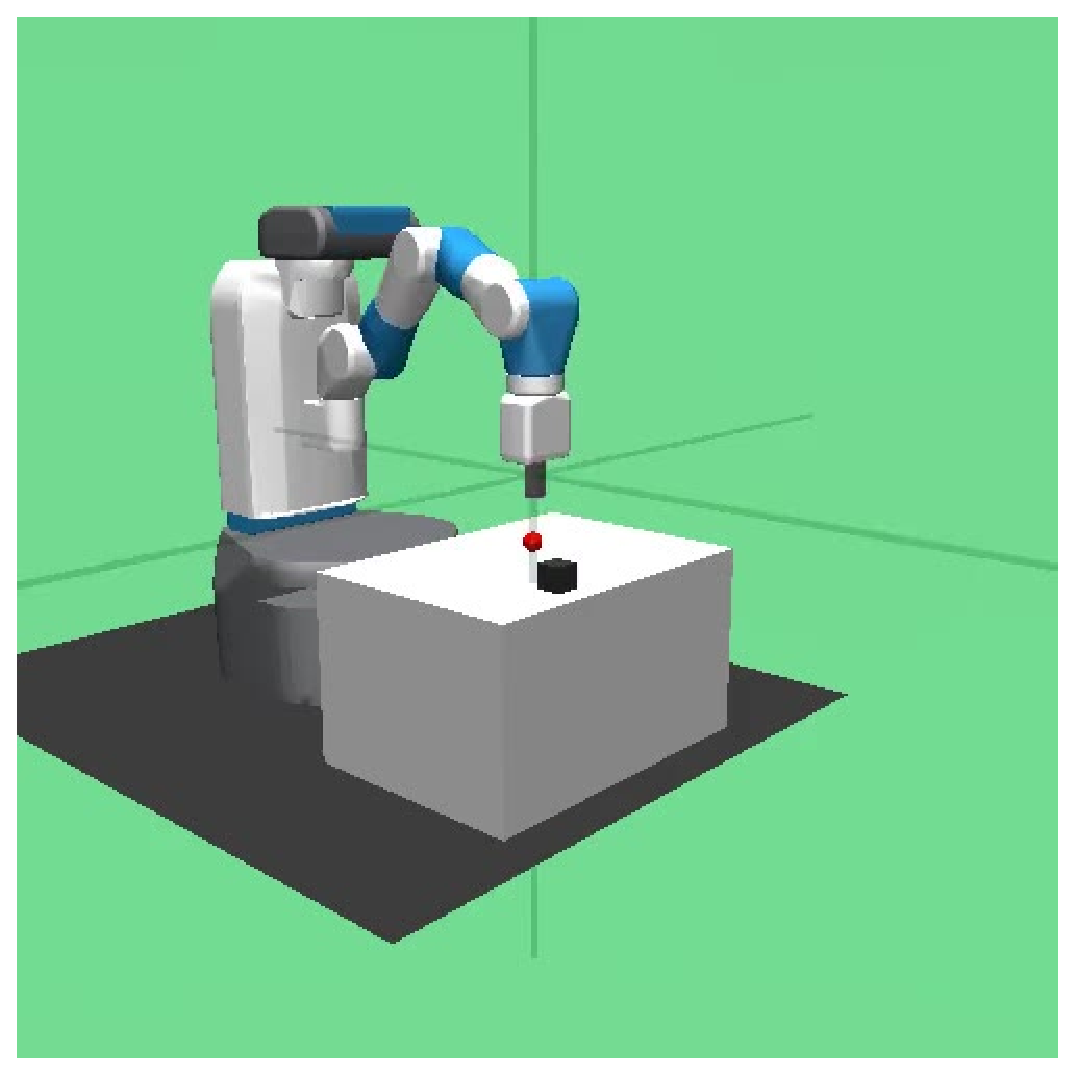
\includegraphics[width=0.3\textwidth]{./fig/fetchpush}
    \label{subfig:fetchpush}
   }
  \subfigure[FetchPickAndPlace.]
   {
    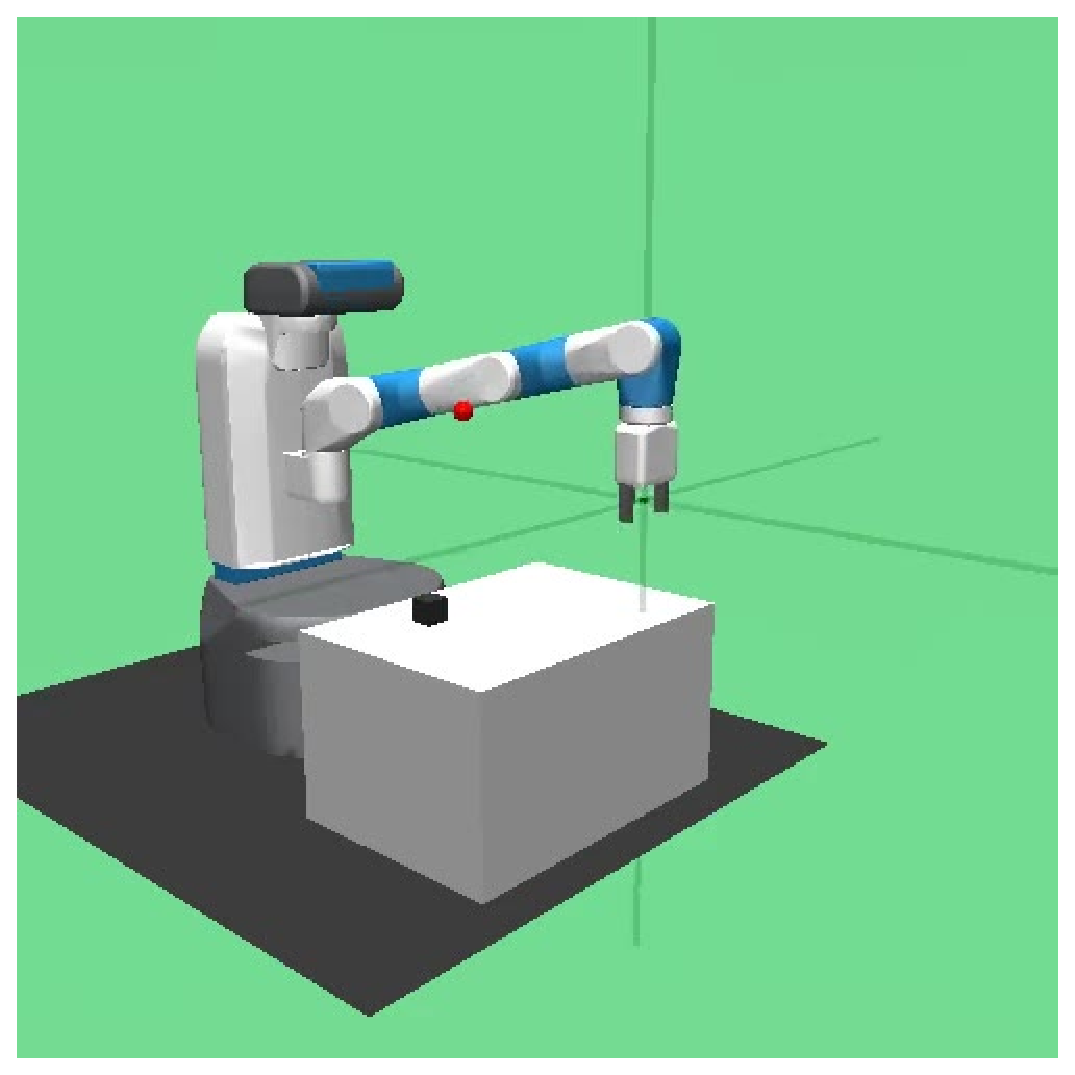
\includegraphics[width=0.3\textwidth]{./fig/fetchpickandplace}
    \label{subfig:fetchpickandplace}
   }
   \captionsetup{width=1\textwidth}
   \caption{Ambientes de manipulação selecionados.}
  \label{fig:fetchenvs}
\end{figure}

Em \textit{FetchReach} (Figura \ref{subfig:fetchreach}) o agente deve posicionar a garra no alvo representado pela esfera vermelha. Em \textit{FecthPickAndPlace} (Figura \ref{subfig:fetchpickandplace}) o agente deve pegar o disco com a garra e posicioná-lo no alvo. Em \textit{FetchPush} (Figura \ref{subfig:fetchpush}) o agente deve empurrar o disco para o alvo.

A recompensa nestes ambientes é considerada, neste trabalho, sendo -1 para todo passo de simulação onde o agente não resolveu a tarefa e 0 quando a tarefa é resolvida. O episódio é limitado a 2048 passos de simulação e é finalizado assim que o agente alcança o objetivo. A observação do ambiente é composta pela posição, rotação e velocidade das juntas do manipulador, assim como posição, rotação e velocidade do disco e a posição do alvo. A ação de um agente neste ambiente é um vetor composto por 4 componentes que representam o torque em cada atuador do manipulador, desde cada junta até a abertura da garra.

% - - - - - - - - - - - - - - - - - - - - - - - - - - - - - - - - - - -

\section{Algoritmo PPO com Motivação Intrínseca}
\label{sec:algoritmo}

O algoritmo utilizado adiciona um passo adicional no funcionamento padrão do PPO descrito em \cite{achiam} e é representado pelo Algoritmo \ref{alg:ppocuriosity} e pela Figura \ref{fig:ppomotivated}. Os passos são descritos com maiores detalhes logo em seguida.

\medskip
\begin{center}
\begin{minipage}{0.92\textwidth}
\begin{algorithm2e}[H]
 \DontPrintSemicolon
 \Entrada{parâmetros da política inicial $\theta_0$, limiar de corte $\epsilon$}
 \Para{$k= 0, 1, 2, ...$} {
    Colete um conjunto de trajetórias $D_k$ com política $\pi_k = \pi(\theta_{k})$ \\
    \Para{cada tupla $(s_t, a_t, r_t, s_{t+1})$ em $D_k$} {
        Calcule o erro do modelo de futuro como mostra a Equação \ref{eqn:curiosityloss} \\
        Calcule a recompensa total $r_t$, como mostra a Equação \ref{eqn:curiosityreward}
    }
    Estime a função de vantagem $A_{t}^{GAE(\gamma, \lambda)}$ \\
    Calcule a atualização da política \\
    \hspace{2cm}$\theta_{k+1} = arg \max_{\theta} L^{CLIP + VF + H}(\theta_k)$ \\
    executando N passos do gradiente ascendente, onde \\
    \hspace{2cm}$L^{CLIP + VF + H}(\theta_k) = \mathop{{}\mathbb{E}}{}_t [L^{CLIP} - L^{VF} + cH(\pi(s_t; \theta))]$ 
 }
\caption{PPO com motivação intrínseca \label{alg:ppocuriosity} }
\end{algorithm2e}
\end{minipage}
\end{center}

Durante a coleta de trajetórias, uma observação $s_t$ do ambiente é passada para o agente a cada passo $t$ de simulação. Essa observação é então alimentada em duas redes neurais: uma rede que calcula a ação $a_t$ a ser tomada, chamada de ator, e uma rede que calcula o valor do estado atual, chamada de crítico. Após a seleção da ação, esta é executada e obtém-se a observação do estado $s_{t+1}$ e a recompensa extrínseca do ambiente. Após o passo de coleta de trajetórias, a recompensa intrínseca é calculada alimentando o modelo de futuro com $(s_t, a_t)$ e calculando o erro $L_F(s_t+1, \hat{s}_{t+1})$. Ao final do episódio o valor da função de vantagem é calculado, os parâmetros do ator são atualizados de acordo com a Equação \ref{eqn:totalloss}, os parâmetros do modelo de futuro são atualizado de acordo com a Equação \ref{eqn:curiosityloss} e os parâmetros do crítico são atualizados de acordo com o erro quadrático médio entre os valores dos estados previstos pela rede e os reais valores obtidos no episódio.

\begin{figure}[ht]
 \centering
  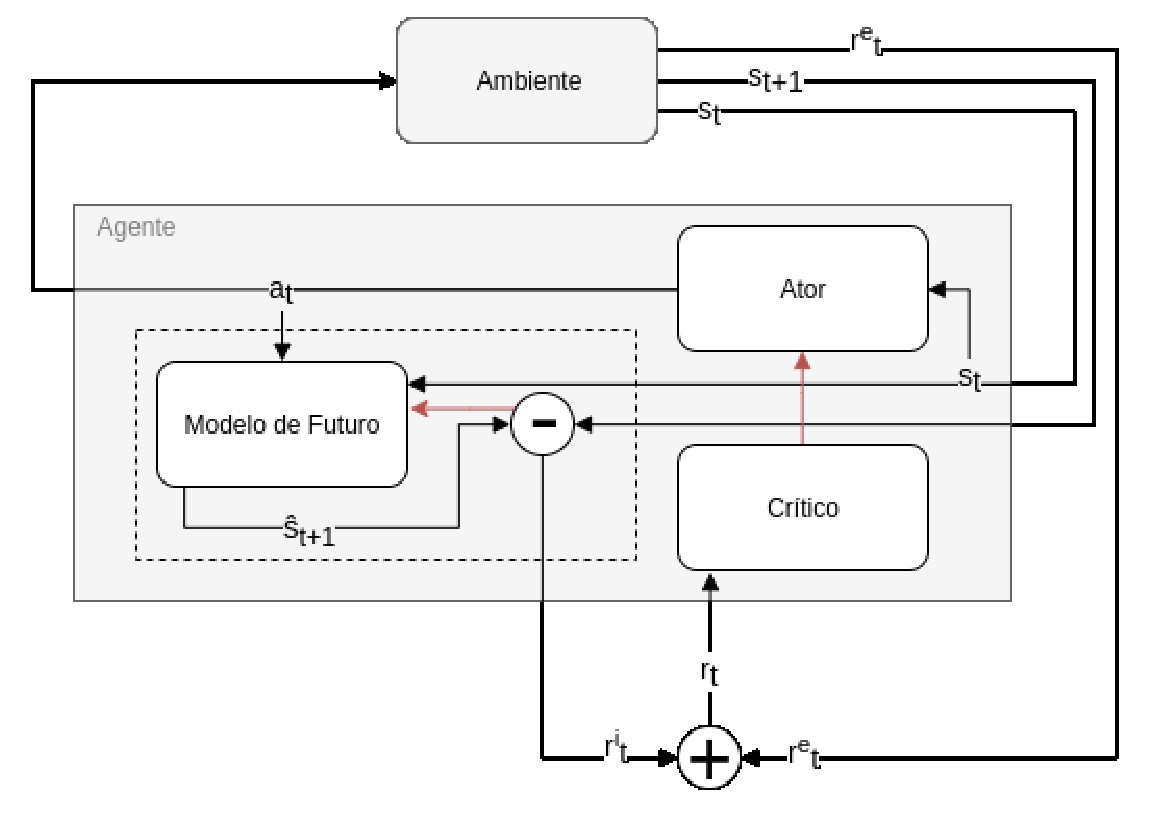
\includegraphics[width=0.70\textwidth]{./fig/ppomotivateddiagram}
  \captionsetup{width=1\textwidth}
  \caption[Diagrama do funcionamento do algoritmo PPO com motivação intrínseca com modelo Ator-Crítico.]{Diagrama do funcionamento do algoritmo PPO com motivação intrínseca com modelo Ator-Crítico. As setas pretas representam os fluxos dos dados no passo de coleta de trajetórias e as setas vermelhas representam o fluxo dos dados no passo de otimização.}
 \label{fig:ppomotivated}
\end{figure}

A rede neural do ator possui duas camadas densas com 128 neurônios cada e função de ativação ReLU, uma terceira camada densa com 15 neurônios e função de ativação TanH e uma camada densa final que tem por objetivo determinar a média $\mu$ da distribuição de probabilidades da saída. O desvio padrão $\sigma$ da distribuição é determinada por parâmetros aprendidos pelo próprio modelo e tende a ser controlado a fim de manter a entropia da distribuição alta enquanto for possível \cite{williamspeng}. A ação do agente é selecionada fazendo a amostragem da distribuição $N(\mu, \sigma^2)$. A rede neural do crítico possui uma topologia semelhante a do ator nas duas primeiras camadas mas sua camada de saída possui apenas um neurônio. A configuração detalhada dos hiperparâmetros do algoritmo utilizado nos experimentos pode ser conferida no Apêndice \ref{apend:1}.

% - - - - - - - - - - - - - - - - - - - - - - - - - - - - - - - - - - -

\section{Testes}
\label{sec:testes}

Os testes são executados de forma a analisar o impacto da motivação intrínseca no aprendizado por reforço em ambientes de manipulação robótica com recompensa esparsa. Para isso, o treinamento do agente é executado nas mesmas condições em dois testes, onde no primeiro a recompensa intrínseca é adicionada à recompensa total e na segunda somente a recompensa extrínseca é transmitida. Para cada teste, o agente foi treinado no ambiente \textit{FetchReach} por 10 milhões de iterações iterações e nos ambientes \textit{FetchPush} e \textit{FetchPickAndPlace} por 30 milhões de iterações. Os testes foram executados paralelamente em seis máquinas com dez núcleos de processamento cada e sem GPUs, resultando em um tempo de treinamento total de aproximadamente oito horas. Os resultados são obtidos durante o processo de treinamento através da ferramenta Tensorboard\footnote{Disponível em \url{https://www.tensorflow.org/tensorboard/get\_started}}.

Como métrica de desempenho é analisada a porcentagem de sucessos em cada lote de avaliações durante o treinamento de cada tarefa, assim como a recompensa intrínseca média, a entropia da política e a divergência KL entre as políticas de antes e depois de uma atualização de parâmetros. A taxa de sucesso mostra a eficiência do algoritmo em alcançar o objetivo e se isso ocorre de forma consistente. A recompensa intrínseca mostra como o modelo de futuro se comporta ao se deparar com os diversos estados em que o agente se encontra durante o treino e testa sua capacidade de predição, ou seja, o entendimento da dinâmica do ambiente. Picos no gráfico de recompensa intrínseca podem indicar aumento do interesse do agente sobre alguma situação específica que modificou o padrão das observações do ambiente de forma significativa. A entropia da política indica quão conservador o agente é em relação a probabilidade de escolha entre as ações, ou seja, se o mesmo permite que diferentes sequências de ações sejam tomadas para atingir seus objetivos. Altos valores de entropia da política podem indicar boas capacidades de generalização, uma vez que mostra que o agente não só simplesmente "decorou" uma sequência específica de ações que resolve o objetivo \cite{williamspeng}. A divergência KL mostra o ritmo no qual a política se modifica entre as atualizações. Esse ritmo tende a ser alto em fases do treinamento em que o agente está modificando significativamente sua política e pode estar relacionado com quedas ou aumentos em sua taxa de sucesso.

Como hipótese, é esperado que o agente com recompensa intrínseca se saia melhor que o algoritmo sem a mesma, refletindo na razão de sucessos máxima de ambos e na velocidade em que se estabilizam nesta métrica. Além disso, espera-se picos de recompensa intrínseca quando mudanças de comportamento do agente influenciam diferentes aspectos da observação no ambiente.